\section{Introduction}
\label{sec:intro}

% \figgray{\bm{$z_s$}}


\begin{figure}
    \centering
    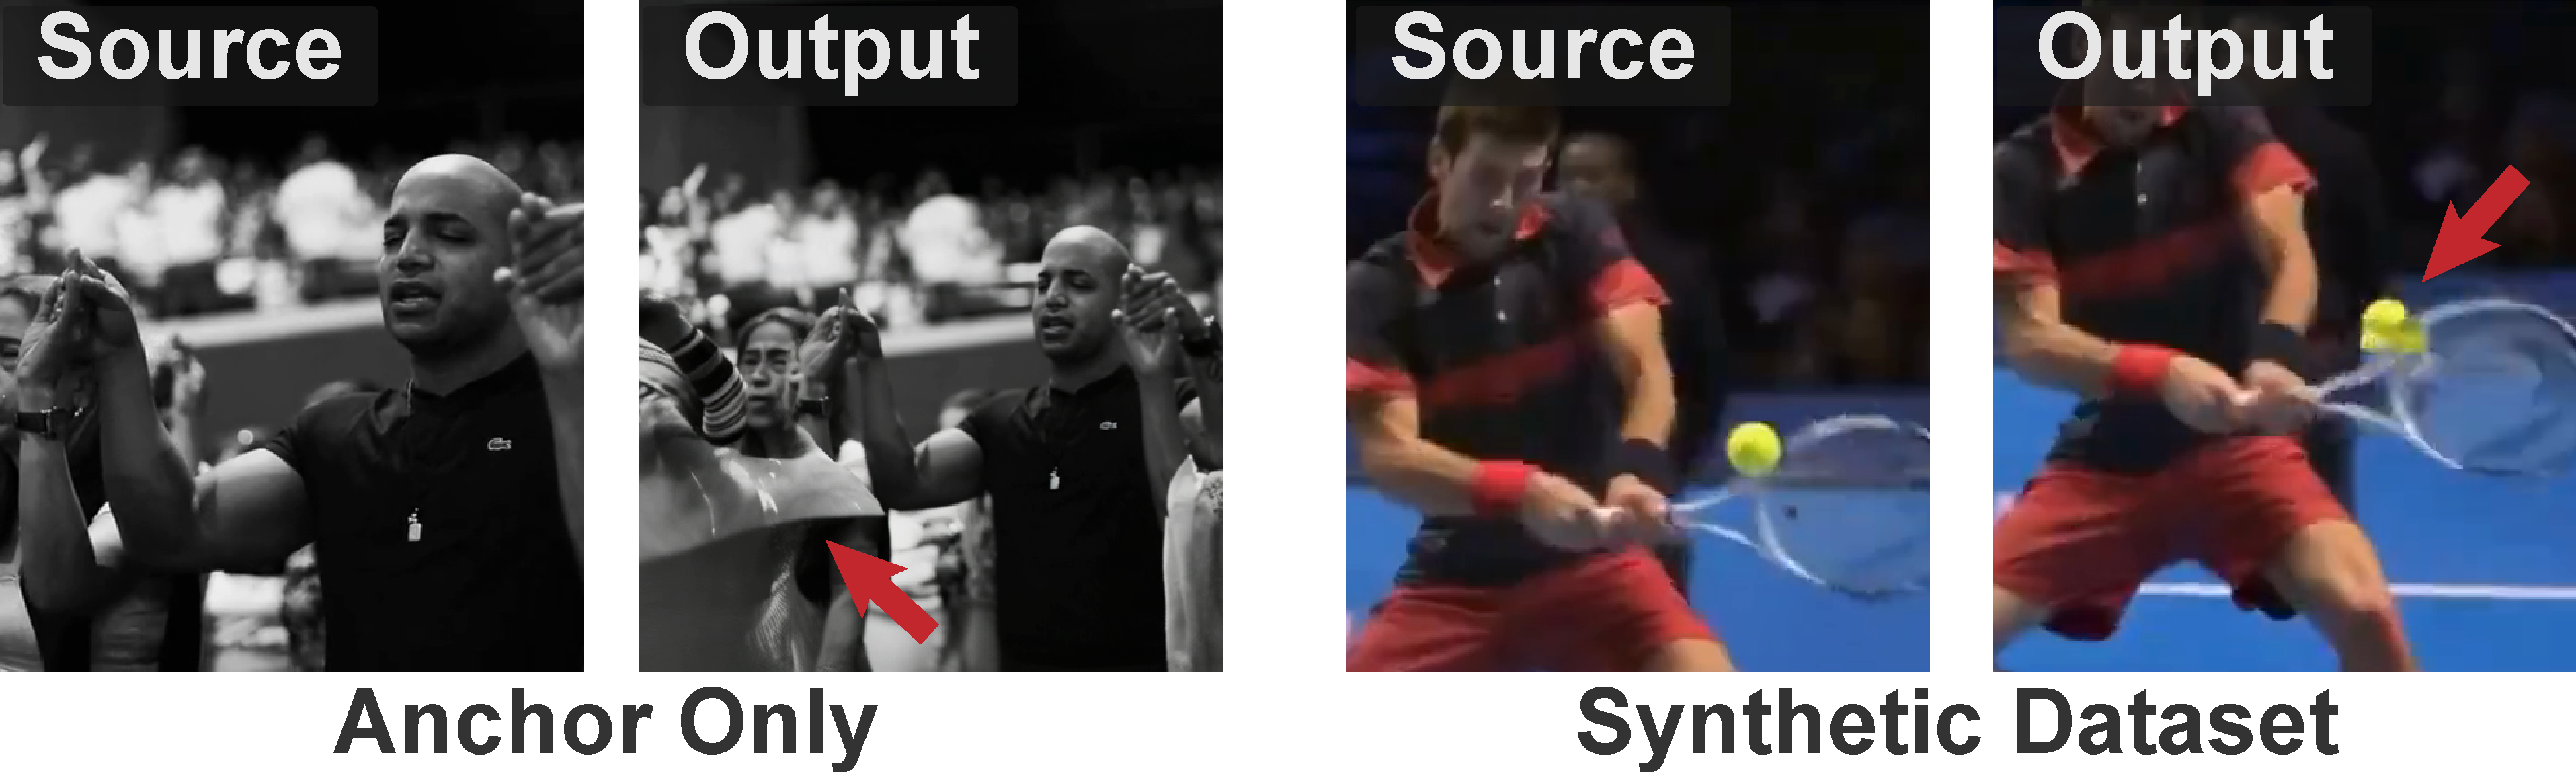
\includegraphics[width=\linewidth]{figures/motivation.pdf}
    \vspace{-0.25in}
    \caption{A comparison of video reshooting challenges. (a) Anchor-only methods~\cite{ex4d} are prone to artifacts when the anchor video $V_a$ is of low quality. (b) Synthetic data trained models~\cite{bai2025recammaster} can fail to generalize and may produce artifacts on unseen interactions, like a tennis ball being hit.}
    \label{fig:motivation}
    \vspace{-0.2in}
\end{figure}



Cinematic camera movement is a vital tool for enriching visual storytelling, as it shapes the audience's perception, deepening emotional impact and clarifying narrative intent. Precise camera framing emphasizes a subject and establishes the spatial context and scope of a scene. However, achieving this level of professional-grade cinematography is often restricted by the significant cost of hardware, technical proficiency and physical constraints of the original shoot. The process of video re-shooting offers an accessible and powerful solution by employing algorithms to digitally modify camera trajectories in post-production, empowering creators to retrofit their existing footage with more refined and compelling camera dynamics.

A primary obstacle to developing robust video re-shooting models is the lack of large-scale, paired multi-view video data. To circumvent this, most existing approaches fall into two categories. First, some methods rely on large-scale synthetic datasets~\cite{bai2025recammaster, gcd}. While useful, the synthetic-to-real generalization gap is notoriously difficult to bridge; a model trained on rendered graphics struggles to generalize to the diverse domains of photorealistic video, animation, gaming, or abstract generative art. As illustrated in Figure~\ref{fig:motivation}(b), such models~\cite{ex4d} can also fail to generalize to complex or novel object interactions not seen in their training distribution, often producing significant visual artifacts.

Second, other methods attempt to build complex 4D representations from pretrained 3D/4D models~\cite{4d_recon_harley2025alltracker,4d_recon_hu2025depthcrafter,4d_recon_wang2024dust3r}. The simplest of these, such as~\cite{ex4d}, operate as \textit{anchor-only models}. As shown in Figure~\ref{fig:motivation}(a), this approach is highly vulnerable to errors in the 3D/4D reconstruction, as any artifacts in the anchor video are propagated to the final output. More advanced techniques, like \trajectorycrafter{}~\cite{yu2025trajectorycrafter}, attempt to mitigate this by using the original source video as an additional input. However, all of these 3D/4D-based approaches are still fundamentally constrained by the limited quality and high computational cost of their underlying 3D/4D data pipelines.

In this paper, we propose a fundamentally different approach that requires no multi-view hardware, 3D annotations, or synthetic data. Our core idea is a novel self-supervised strategy for generating a \textit{pseudo multi-view training triplet}—consisting of a source, anchor, and target video—from a single monocular video. We first extract two distinct clips to serve as the \textit{source video} and the \textit{target video}, using \textit{smooth random walk trajectories} that simulate dynamic camera motion. We then synthetically generate the \textit{anchor video} by warping the first frame of the source video using a dense 2D tracker and a forward warping technique, which effectively simulates the distorted point-cloud-based inputs we expect at inference.

This training setup forces the model to learn a robust, 3D-aware understanding of scene dynamics. To reconstruct the target video, the model must learn to ignore artifacts in the anchor video and retrieve the correct texture from the source video. Crucially, to fill dis-occluded regions in the target, the model is compelled to find the missing texture in a different temporal context in the source video (e.g., from a later frame), forcing it to perform implicit 3D reasoning by re-projecting content across different times and pseudo-viewpoints.

Our contributions are three-fold:
\begin{itemize}[noitemsep, topsep=0pt, partopsep=0pt]
    \item First, we introduce a highly scalable and domain-agnostic self-supervised data pipeline that generates (source, anchor, target) training triplets from any monocular video.
    \item Second, we propose a \textit{minimal and efficient architectural adaptation} that leverages a pre-trained model's existing temporal modules, avoiding the instability of introducing complex architectural changes.
    \item Third, we demonstrate through extensive experiments that our approach achieves state-of-the-art temporal consistency and camera control across a diverse set of videos, significantly advancing the capabilities of video re-shooting.
\end{itemize}